\chapter{Đánh giá hệ thống}\label{chap4}
\section{Hiệu quả hoạt động}\label{sec:efficiency}
Nhằm đánh giá tính hiệu quả của phương pháp đề xuất, khóa luận đã cài đặt một số mô-đun và tích hợp phương pháp đề xuất trên công cụ AKAUTAUTO và thực hiện thực nghiệm trên công cụ này. AKAUTAUTO là một công cụ kiểm thử tự động cho mã nguồn C/C++, được nghiên cứu và phát triển bởi Phòng thí nghiệm Đảm bảo chất lượng phần mềm (Khoa Công nghệ thông tin, Trường Đại học Công nghệ, ĐHQGHN) và đơn vị FPT-GAM (FPT Global Automative \& Manufacturing). Khóa luận kế thừa kiến trúc của công cụ AKAUTAUTO phiên bản 5.9.2, phiên bản tích hợp sẵn phương pháp kiểm thử tượng trưng động và phương pháp sinh giả lập mã nguồn tự động AS4UT, và bổ sung, cải tiến một số mô-đun trong kiến trúc gốc để tích hợp phương pháp đề xuất (phiên bản 5.9.2-thesis).

% \subsection{Tổng quan kiến trúc công cụ AKAUTAUTO}
Công cụ AKUTAUTO được phát triển bằng ngôn ngữ Java với kiến trúc bao gồm sáu mô-đun chính lần lượt là mô-đun xây dựng môi trường kiểm thử, mô-đun phân tích mã nguồn, mô-đun xử lý hàm thiếu định nghĩa, mô-đun sinh dữ liệu kiểm thử, mô-đun thực thi \& phân tích ca kiểm thử và mô-đun sinh báo cáo kiểm thử. Hình \ref{fig:architect} mô tả kiến trúc của công cụ AKAUTAUTO gồm sáu mô-đun kể trên và các thành phần ngoài gồm trình biên dịch C/C++, bộ giải Z3 và thư viện phân tích mã nguồn CDT Parser. Trong đó, khóa luận đã bổ sung mô-đun xử lý hàm thiếu định nghĩa so với kiến trúc gốc, và cải tiến hai mô-đun phân tích mã nguồn và mô-đun sinh dữ liệu kiểm thử (thể hiện bởi các khối in đậm).

\begin{figure}[t]
    \centering
    \includesvg[width=\linewidth]{images/architect.svg}
    \caption{Kiến trúc công cụ AKAUTAUTO.}
    \label{fig:architect}
\end{figure}

Đầu vào của công cụ AKAUTAUTO gồm hai thành phần chính lần lượt là các tệp mã nguồn kiểm thử và cấu hình kiểm thử. Hai thành phần này được cung cấp bởi kiểm thử viên hoặc lập trình viên. Mô-đun xây dựng môi trường kiểm thử là mô-đun tiếp nhận các thành phần đầu vào và đảm nhiệm vai trò thực hiện hai tác vụ tiền xử lý mã nguồn trong pha xây dựng môi trường kiểm thử. Hai tác vụ tiền xử lý đã được đề cập ở Mục~\ref{sec:3-build-env} gồm thiết lập môi trường và tạo môi trường tính toán độ phủ. Mô-đun xây dựng môi trường kiểm thử cấu thành bởi ba thành phần chính đó là thành phần thiết lập môi trường, thành phần tải dự án và thành phần tạo môi trường tính toán độ phủ. Trong đó, hai thành phần thiết lập môi trường và tạo môi trường tính toán độ phủ thực hiện hai tác vụ tương ứng đã nêu. Thành phần tải dự án có nhiệm vụ xác định các tệp mã nguồn được người dùng thiết lập, sau đó kiến tạo đỉnh tệp của từng cây cấu trúc tệp tương ứng. Đầu ra của mô-đun gồm các tệp mã nguồn đã được thêm lệnh đánh dấu và tập các cây cấu trúc tệp cơ bản sinh bởi thành phần tải dự án. Các tệp mã nguồn chứa lệnh đánh dấu sẽ được sử dụng bởi mô-đun xử lý hàm thiếu định nghĩa nhằm sinh thân hàm giả trên tệp mã nguồn này. Tập cây cấu trúc tệp cơ bản và mã nguồn gốc sẽ được phân tích bởi mô-đun phân tích mã nguồn.

Các mô-đun tiếp theo trong kiến trúc của công cụ AKAUTAUTO được khóa luận bổ sung hoặc cải tiến gồm mô-đun phân tích mã nguồn, mô-đun xử lý hàm thiếu định nghĩa và mô-đun sinh dữ liệu kiểm thử. Chi tiết về sự cải tiến của mô-đun phân tích mã nguồn và mô-đun sinh dữ liệu kiểm thử được trình bày lần lượt ở Mục~\ref{sec:module-analyze} và Mục~\ref{sec:module-autogen}. Mô-đun xử lý hàm thiếu định nghĩa được bổ sung so với kiến trúc gốc nhằm giải quyết các vấn đề phát sinh bởi nguyên mẫu hàm thiếu định nghĩa. Nội dung chi tiết của mô-đun này được trình bày ở Mục~\ref{sec:module-undef}. 

Khóa luận kế thừa mô-đun thực thi và phân tích ca kiểm thử từ kiến trúc gốc của công cụ. Mô-đun này đóng vai trò  sinh trình điều khiển kiểm thử, thực thi trình điều khiển và phân tích đường thi hành thu được sau khi chạy ca kiểm thử. Cấu trúc của mô-đun gồm ba thành phần chính với nhiệm vụ chi tiết của từng thành phần như sau:
\begin{itemize}
    \item Thành phần sinh trình điều khiển kiểm thử: Đảm nhiệm hai vai trò chuyển đổi bộ nghiệm giải từ ràng buộc thành dữ liệu kiểm thử C++ và sinh trình điều khiển kiểm thử dựa trên dữ liệu mới. Trình điều khiển kiểm thử là một tệp C++ được tự động sinh ra nhằm chuyển đổi dữ liệu kiểm thử C++ thành các cú pháp C++ giúp khởi tạo giá trị tham số đầu vào của đơn vị kiểm thử. Các cú pháp C++ trong trình điều khiển gồm hai phần chính đó là phần định nghĩa tham số đầu vào và phần gọi đơn vị kiểm thử. Trình điều khiển cũng đảm nhiệm chuyển hóa dữ liệu kiểm thử C++ thành các mã nguồn giả lập cho các hàm cần stub.
    \item Thành phần thực thi ca kiểm thử: Có nhiệm vụ biên dịch trình điều khiển và các tệp mã nguồn chứa lệnh đánh dấu thành tệp đối tượng rồi sau đó liên kết các tệp này để tạo thành tệp thực thi. Công cụ chạy tệp thực thi này và thu được danh sách các câu lệnh, các nhánh điều kiện được viếng thăm bởi ca kiểm thử.
    \item Thành phần phân tích đường thi hành: Có chức năng ánh xạ danh sách các câu lệnh, nhánh điều kiện được viếng thăm sang đỉnh tương ứng trong CFG của đơn vị kiểm thử. Tiếp đó, thành phần cập nhật dữ liệu viếng thăm của CFG dựa trên tập đỉnh được ánh xạ. Cuối cùng, thành phần phân tích đường thi hành sẽ tìm đường thi hành ngắn nhất chưa được viếng thăm và truyền đường thi hành này sang mô-đun sinh dữ liệu kiểm thử.
\end{itemize}

Mô-đun cuối cùng trong kiến trúc công cụ là mô-đun sinh báo cáo kiểm thử. Mô-đun này có vai trò tính toán độ phủ của đơn vị kiểm thử dựa trên dữ liệu viếng thăm của CFG và tạo báo cáo kiểm thử sau khi quá trình sinh dữ liệu kiểm thử tự động kết thúc. Hình \ref{fig:report} mô tả ví dụ báo cáo kiểm thử LCOV của hàm \tcode{foo}. Khóa luận đã sinh dữ liệu kiểm thử tự động cho hàm \tcode{foo} và đạt được độ phủ 100\% câu lệnh cũng như 100\% nhánh với ba ca kiểm thử. Các thông tin ở góc trên phải của báo cáo cho biết 7/20 dòng lệnh của tệp chứa hàm \tcode{foo} và 4/4 nhánh điều kiện có trong hàm được thăm bởi ba ca kiểm thử này. 

\begin{figure}[h]
    \centering
    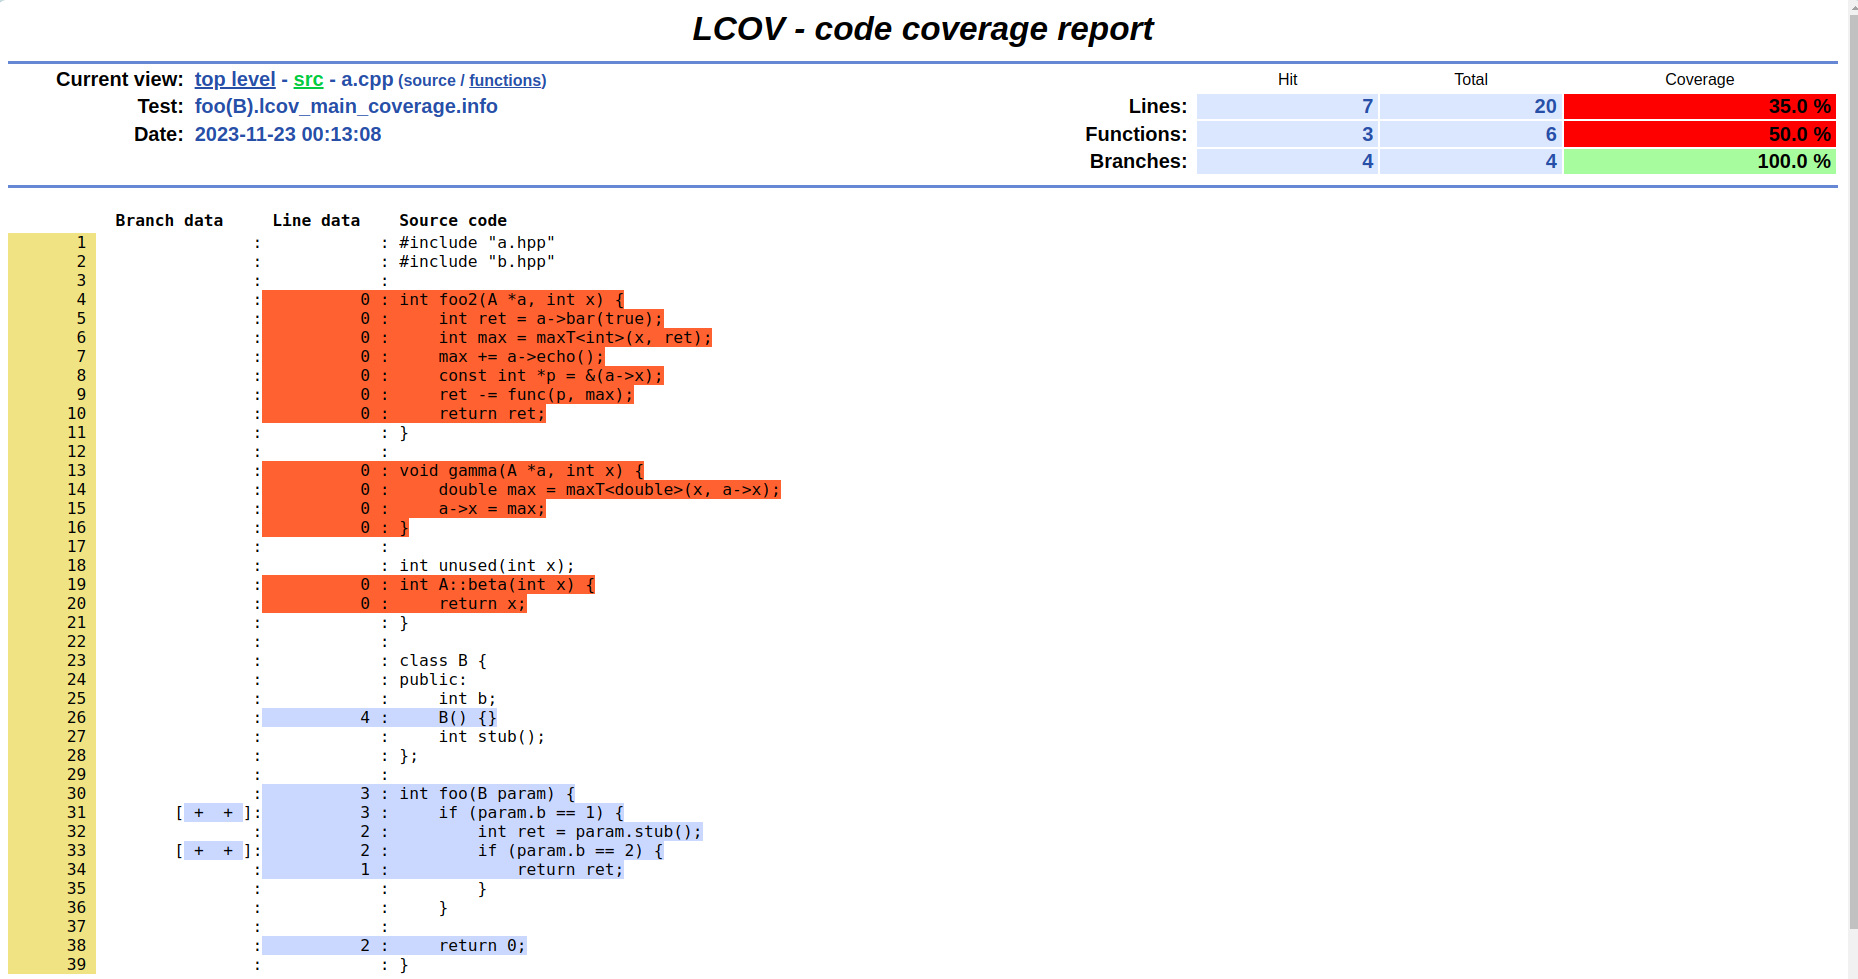
\includegraphics[width=\linewidth]{images/report.png}
    \caption{Báo cáo kiểm thử LCOV của hàm \tcode{foo}.}
    \label{fig:report}
\end{figure}

% \begin{figure}
%     \centering
%     \includesvg[width=0.8\linewidth]{images/module-build.svg}
%     \caption{Các thành phần trong mô-đun xây dựng môi trường kiểm thử.}
%     \label{fig:module-build}
% \end{figure}

% Đầu vào của mô-đun xây dựng môi trường kiểm thử gồm tập mã nguồn kiểm thử và tệp cấu hình kiểm thử được người dùng thiết lập thông qua giao diện của công cụ. Đoạn~mã~\ref{cod:enviro} minh họa tệp cấu hình kiểm thử đầu vào. Dòng 2-11 trong đoạn mã cho biết môi trường kiểm thử sử dụng trình biên dịch GNU mặc định của máy kèm theo một số câu lệnh cơ bản để biên dịch mã nguồn kiểm thử. Dòng 12-14 cho biết thêm thông tin về tên của môi trường kiểm thử, phương pháp kiểm thử cũng như loại độ phủ sẽ được tính là gì. Môi trường ví dụ có tên là \tcode{auto-sample}, sử dụng phương pháp kiểm thử tự động đề xuất bởi khóa luận và hai kiểu độ phủ được tính là độ phủ câu lệnh và độ phủ MCDC. Tệp cấu hình kiểm thử được lưu lại nhằm phục vụ cho các lần kiểm thử sau trên cùng môi trường \tcode{auto-sample}. 
% \begin{figure}[h]
% \begin{lstlisting}[language={}, caption={Tệp cấu hình kiểm thử.}, captionpos=b, label={cod:enviro}]
% ENVIRO.NEW
% ENVIRO.COMPILER.NEW
% ENVIRO.COMPILER.NAME: [GNU Native] C++
% ENVIRO.COMPILER.COMPILE_CMD: g++ -c -w
% ENVIRO.COMPILER.PREPROCESS_CMD: g++ -c -E
% ENVIRO.COMPILER.LINK_CMD: g++ -w
% ENVIRO.COMPILER.INCLUDE_FLAG: -I
% ENVIRO.COMPILER.DEFINE_FLAG: -D
% ENVIRO.COMPILER.OUTPUT_FLAG: -o
% ENVIRO.COMPILER.OUTPUT_EXT: .out
% ENVIRO.COMPILER.END
% ENVIRO.NAME: auto_sample
% ENVIRO.TESTING_METHOD: PROPOSED-METHOD
% ENVIRO.COVERAGE_TYPE: STATEMENT+MCDC
% ENVIRO.END
% \end{lstlisting}
% \end{figure}
% \subsection{Mô-đun phân tích mã nguồn}\label{sec:module-analyze}
Mô-đun phân tích mã nguồn đảm nhiệm vai trò trích xuất, phân tích thông tin từ AST của mã nguồn kiểm thử, xây dựng đồ thị cấu trúc mã nguồn và cung cấp dịch vụ tìm kiếm thông tin đỉnh trên đồ thị. Hình~\ref{fig:module-analyze} mô tả cấu trúc của mô-đun với ba thành phần lần lượt là thành phần sinh AST, thành phần sinh đồ thị cấu trúc mã nguồn và thành phần tìm kiếm trên đồ thị. Trong đó, khóa luận kế thừa thành phần sinh AST, cải tiến mô-đun sinh đồ thị cấu trúc mã nguồn và bổ sung thành phần tìm kiếm trên đồ thị.
\vspace{5mm}
\begin{figure}[h]
    \centering
    \includesvg[width=0.8\linewidth]{images/module-analyze.svg}
    \caption{Các thành phần trong mô-đun phân tích mã nguồn.}
    \label{fig:module-analyze}
\end{figure}

Mô-đun phân tích mã nguồn nhận đầu vào là mã nguồn kiểm thử gốc và các đỉnh tệp từ đầu ra của mô-đun xây dựng môi trường. Bắt đầu từ mỗi đỉnh tệp, dựa trên quan hệ cha con trên AST của từng tệp mã nguồn, quá trình sinh cây cấu trúc tệp được diễn ra song song. Sau đó, tập cây cấu trúc tệp được chuyển sang thành phần hoàn thiện đồ thị cấu trúc để bổ sung cạnh kế thừa và cạnh lời gọi hàm. Tại thành phần này, từng cây cấu trúc tệp được xét và tìm kiếm các đỉnh có tiêu chí phù hợp với kiểu cạnh đang xét trên các cây cấu trúc còn lại. Kết quả của quá trình xây dựng là đồ thị cấu trúc mã nguồn kiểm thử.

Khóa luận đã cải tiến thành phần sinh đồ thị cấu trúc mã nguồn như sau. Trước hết, khóa luận tích hợp thành phần ánh xạ cây cấu trúc và thành phần phân tích phụ thuộc~\cite{TUNG2022106821} trong kiến trúc gốc thành mô-đun sinh đồ thị cấu trúc mã nguồn. Quá trình tích hợp bổ sung các luồng xử lý song song quá trình sinh cây cấu trúc tệp giúp giảm thời gian phân tích mã nguồn. Sau đó, khóa luận bổ sung các loại đỉnh mới biểu thị cho các kiểu khai báo mới trong ngôn ngữ C++ như không gian tên, câu lệnh sử dụng không gian tên, khai báo lớp không cần tên kiểu, v.v. Qua đó, thành phần này có thể phân tích và biểu diễn được các đặc trưng mới của C++ trên đồ thị cấu trúc mã nguồn.\\

Tìm kiếm thông tin đỉnh trên đồ thị là quá trình cốt lõi phục vụ cho quá trình xử lý hàm thiếu định nghĩa và quá trình sinh dữ liệu kiểm thử tự động. Trong kiến trúc gốc, quá trình tìm kiếm duyệt qua các đỉnh trên đồ thị, kiểm tra thông tin của đỉnh có hợp với tiêu chí tìm kiếm rồi thêm vào tập kết quả nếu hợp lệ. Trong thực tế, đồ thị cấu trúc thường rất lớn. Vậy nên quá trình tìm kiếm tốn nhiều bộ nhớ bởi quá trình đệ quy xuống đỉnh. Để khắc phục nhược điểm này, khóa luận bổ sung thành phần tìm kiếm trên đồ thị với ý tưởng chính dựa trên tìm kiếm kết hợp bảng băm và cơ sở dữ liệu. Việc tìm kiếm thông tin đỉnh thường sử dụng hai tiêu chí đó là tên hàm và tên kiểu. Tận dụng điều này, khóa luận tạo cơ sở dữ liệu lưu trữ thông tin về kiểu và hàm của mã nguồn kiểm thử. Cơ sở dữ liệu gồm hai trường chính đó là $id$ - khóa chính biểu thị mã định danh của hàm hoặc kiểu và $name$ - tên hàm hoặc tên kiểu. Sau quá trình xây dựng đồ thị cấu trúc mã nguồn, mỗi đỉnh trong đồ thị được cấp một mã định danh cố định $id$. Mã định danh này là giá trị băm xâu đường dẫn của đỉnh, trong đó xâu đường dẫn là chuỗi tên các đỉnh trên đường đi từ đỉnh tệp xuống đỉnh đang xét. Khóa luận sử dụng một bảng băm để ánh xạ $id$ và đỉnh sở hữu $id$. Để nhanh chóng tìm kiếm tên trong cơ sở dữ liệu, khóa luận sử dụng hệ quản trị cơ sở dữ liệu SQLite\footnote{https://www.sqlitetutorial.net/sqlite-full-text-search/} với cơ chế FULLTEXT INDEX trên cột $name$. Để tìm kiếm một đỉnh phù hợp, trước hết quá trình tìm kiếm sẽ thu thập các dòng trong cơ sở dữ liệu có chứa tên hàm hoặc tên kiểu, trích xuất $id$ và dựa vào bảng băm để lấy ra đỉnh cần xét. 

Quá trình nghiên cứu, cải tiến mô-đun phân tích mã nguồn tốn nhiều thời gian do số lượng tệp ảnh hưởng bởi mô-đun này là rất lớn (113 tệp ảnh hưởng và 5476 LOC thay đổi). Tuy nhiên, quá trình trên là cần thiết bởi công cụ AKAUTAUTO phiên bản 5.9.2 thường gặp lỗi hết bộ nhớ ảo trong quá trình phân tích mã nguồn khi chạy trên các dự án có kích thước lớn, cấu trúc phức tạp và có nhiều sự tương tác trong các thành phần với nhau. Sau quá trình cải tiến, công cụ AKAUTAUTO phiên bản 5.9.2-thesis đã có thể phân tích được những bộ mã nguồn có kích thước lớn, đồng thời không gặp tình trạng hết bộ nhớ ảo trong quá trình chạy.

% \subsection{Mô-đun xử lý hàm thiếu định nghĩa}\label{sec:module-undef}
Mô-đun xử lý hàm thiếu định nghĩa được khóa luận bổ sung so với kiến trúc gốc nhằm thực hiện nhiệm vụ của pha xử lý hàm thiếu định nghĩa. Hình~\ref{fig:module-undef} mô tả các thành phần cấu thành lên mô-đun gồm thành phần thu thập, thành phần lọc tìm ứng viên, thành phần xử lý nguyên mẫu hàm ảo và thành phần sinh thân hàm giả. Mô-đun xử lý hàm thiếu định nghĩa được thiết kế để xử lý hai loại nguyên mẫu hàm thiếu định nghĩa như đã mô tả ở Mục~\ref{sec:handle-undef}. Chi tiết về các thành phần như sau.
\begin{itemize}
    \item Thành phần thu thập: Đóng vai trò thu thập danh sách các nguyên mẫu hàm thiếu định nghĩa cần sinh thân hàm giả. Thành phần thu thập sử dụng các công cụ tiện ích của trình biên dịch để thu thập danh sách này. Phương pháp thu thập đã được trình bày ở Mục~\ref{sec:handle-undef-first}.
    \item Thành phần xử lý nguyên mẫu hàm ảo: Có chức năng tìm kiếm các nguyên mẫu hàm ảo thiếu định nghĩa sử dụng phương pháp đề xuất ở Mục~\ref{sec:handle-undef-second}. Danh sách các nguyên mẫu hàm ảo tìm được sẽ được truyền sang thành phần lọc tìm ứng viên để xử lý theo Thuật~toán~\ref{alg:handle-virtual-undef}. Các nguyên mẫu hàm ảo còn lại sẽ được sinh cạnh định nghĩa tương ứng với đỉnh biểu thị hàm trong đồ thị cấu trúc.
    \item Thành phần lọc tìm ứng viên: Thực hiện quá trình áp dụng Thuật~toán~\ref{alg:filter-undef} trên danh sách các hàm thiếu định nghĩa trả về bởi thành phần thu thập và các nguyên mẫu hàm ảo thiếu định nghĩa tìm được. Đầu ra của thành phần là danh sách các đỉnh trên đồ thị cấu trúc mã nguồn cần được sinh hàm giả. 
    \item Thành phần sinh thân hàm giả: Đảm nhiệm vai trò sinh thân hàm giả cho danh sách các đỉnh được tổng hợp bởi thành phần lọc tìm ứng viên.
\end{itemize}

\begin{figure}[h]
    \centering
    \includesvg[width=0.8\linewidth]{images/module-undef.svg}
    \caption{Các thành phần trong mô-đun xử lý hàm thiếu định nghĩa.}
    \label{fig:module-undef}
\end{figure}

Đầu ra của mô-đun xử lý hàm thiếu định nghĩa là mã nguồn chứa các câu lệnh đánh dấu đã được bổ sung thân hàm giả cho các nguyên mẫu hàm thiếu định nghĩa. Mã nguồn đã chỉnh sửa này sau đó được sử dụng để tính toán độ phủ khi chạy các ca kiểm thử bởi mô-đun thực thi và phân tích ca kiểm thử.

% \subsection{Mô-đun sinh dữ liệu kiểm thử}\label{sec:module-autogen}
Mục tiêu của mô-đun sinh dữ liệu kiểm thử là tự động tạo ra các ca kiểm thử cho các đơn vị cần kiểm thử. Mô-đun được thiết kế như Hình~\ref{fig:module-autogen} với bốn thành phần lần lượt là thành phần sinh CFG, thành phần sinh dữ liệu kiểm thử ngẫu nhiên, thành phần thực thi tượng trưng và thành phần xử lý lời gọi hàm. Trong đó, thành phần xử lý lời gọi hàm được cải tiến bởi phương pháp đề xuất ở Mục \ref{sec:autostub-obj}, các thành phần còn lại được kế thừa từ kiến trúc gốc. Chi tiết về các thành phần như sau.
\begin{itemize}
    \item Thành phần sinh CFG: Có chức năng xây dựng CFG cho các đơn vị trong mã nguồn.
    \item Thành phần sinh dữ liệu kiểm thử ngẫu nhiên: Đảm nhiệm vai trò sinh các ca kiểm thử với dữ liệu ngẫu nhiên trong pha sinh dữ liệu kiểm thử tự động (mô tả ở Mục~\ref{sec:autogen}). 
    \item Thành phần thực thi tượng trưng: Đóng vai trò thực hiện quá trình thực thi tượng trưng trên đường thi hành chưa được viếng thăm và sinh ra các ràng buộc tạo các điểm quyết định trong đồ thị dòng điều khiển. Sau đó, thành phần thực thi tượng trưng sử dụng bộ giải Z3 để giải các ràng buộc và tạo ra các giá trị đầu vào mới.
    \item Thành phần xử lý lời gọi hàm: Có nhiệm vụ tạo giả lập mã nguồn tự động cho các lời gọi hàm xuất hiện trong đường thi hành. Khóa luận kế thừa thành phần xử lý lời gọi hàm dựa trên phương pháp AS4UT và áp dụng phương pháp xử lý lời gọi phương thức được đề xuất ở Mục \ref{sec:autostub-obj}. Đầu ra của thành phần là các thay đổi cần thiết trên CFG, bảng $MAP$ và $REF$ để giúp quá trình thực thi tượng trưng sinh ra bộ dữ liệu kiểm thử mới cho đường thi hành chưa viếng thăm.
\end{itemize}

\begin{figure}[h]
    \centering
    \includesvg[width=0.6\linewidth]{images/module-autogen.svg}
    \caption{Các thành phần trong mô-đun sinh dữ liệu kiểm thử.}
    \label{fig:module-autogen}
\end{figure}
% % \subsection{Mô-đun thực thi và phân tích ca kiểm thử}
% \begin{figure}
%     \centering
%     \includesvg[width=0.8\linewidth]{images/module-execute.svg}
%     \caption{Các thành phần trong mô-đun thực thi và phân tích ca kiểm thử.}
%     \label{fig:module-execute}
% \end{figure}

% Đoạn mã \ref{cod:driver} minh họa ví dụ trình điều khiển kiểm thử sinh bởi mô-đun khi kiểm thử hàm \tcode{foo} trong Đoạn~mã~\ref{cod:autostub-object}. Dòng đầu tiên trong trình điều khiển dùng để thiết lập tên đơn vị kiểm thử, giúp các hàm được stub biết cần phải chạy mã nguồn giả lập nào (mô tả trong Đoạn~mã~\ref{cod:stub-final}). Dòng 2-3 định nghĩa tham số đầu vào \tcode{param} của hàm \tcode{foo} là một đối tượng của lớp \tcode{B} với thuộc tính \tcode{b} có giá trị 1. Dòng 4 trong trình điều khiển dùng để gọi hàm \tcode{foo} với các định nghĩa tham số được khai báo ở trên. Kết quả viếng thăm sau quá trình chạy ca kiểm thử được mô tả bởi Đoạn~mã~\ref{cod:visited}. Kết quả viếng thăm cho biết các dòng 8, 9, 10, 11 và nhánh đúng của biểu thức điều kiện ở dòng 8, 10 trong hàm \tcode{foo} được thăm. \\

% \begin{figure}[h]
%     \begin{minipage}[t]{0.5\linewidth}
%     \begin{lstlisting}[language={C++}, caption={Trình điều khiển kiểm thử cho Đoạn mã \ref{cod:autostub-object}.}, captionpos=b, label={cod:driver}]
% TEST_CASE_NAME = "foo";
% B param;
% param.b = 1;
% int AKA_ACTUAL_OUTPUT = foo(param);
%     \end{lstlisting}
%     \end{minipage}
%     \begin{minipage}[t]{0.5\linewidth}
%     \begin{lstlisting}[language=C++, caption={Danh sách các câu lệnh và nhánh điều kiện được thăm bởi trình điều khiển.}, label={cod:visited}, captionpos=b]
% visit_line_8
% visit_condition_1_T
% visit_line_9
% visit_line_10
% visit_condition_1_T
% visit_line_11
%     \end{lstlisting}
% \end{minipage}
% \end{figure}
\section{Các vấn đề gặp phải}\label{sec:problem}